\section{Does the combined manifold cure non-renormalizability?}
\label{sec:renorm}

\subsection{Power counting}

With $\hbar=1$ and the speed of light 1, every quantity has a mass dimension, written in square
brackets. Let $D$ be the number of space dimensions in which the fields carry momentum (the symbol of
the project with this meaning): $D=7$ on the eight-dimensional spacetimes, $D=3$ in the
four-dimensional world. The action is dimensionless, so the Lagrangian density has dimension $D+1$,
and its kinetic terms fix the dimension of a fermion field to $D/2$ and of a scalar or gauge field to
$(D-1)/2$. The couplings then have the dimensions of Table~\ref{tab:powercount}: a gauge or Yukawa
coupling $(3-D)/2$, a quartic scalar coupling $3-D$, and a four-fermion contact coupling, such as
$G_{\rm NG}$ of Eq.~(\ref{eq:hv}), $1-D$ (check R-1). For $D=7$ every interaction has a coupling of
negative mass dimension.

\begin{table}[t]
\caption{Mass dimensions of fields and couplings for $D$ space dimensions (exact; data
\texttt{data/ng\_power\_counting.csv}).}
\label{tab:powercount}
\begin{ruledtabular}
\begin{tabular}{lccc}
& general $D$ & $D=3$ & $D=7$\\
\hline
{{GENRAW:power_rows}}
\end{tabular}
\end{ruledtabular}
\end{table}

A coupling of negative dimension makes a theory non-renormalizable: the superficial degree of
divergence of a one-particle-irreducible graph, the power of the cutoff with which the graph grows
when all its loop momenta are large, is
\begin{align}
\deg_{\rm NG}&=(D+1)-\frac D2e^{\rm F}_{\rm NG}-\frac{D-1}2e^{\rm B}_{\rm NG}\nonumber\\
&\quad-\sum_{\rm vertices}[\text{coupling of the vertex}],
\label{eq:degree}
\end{align}
with $e^{\rm F}_{\rm NG}$ and $e^{\rm B}_{\rm NG}$ the numbers of external fermion and boson lines; it
grows without bound with the number of vertices when a coupling has negative dimension, and infinitely
many counterterms are needed. For the four-point function of the four-fermion interaction
($e^{\rm F}_{\rm NG}=4$, $e^{\rm B}_{\rm NG}=0$) with $\mathcal V_{\rm NG}$ vertices, Eq.~(\ref{eq:degree})
gives $\deg_{\rm NG}=(\mathcal V_{\rm NG}-1)(D-1)$: for $D=3$ it is 2 at one loop---the quadratic
growth with $\Lambda_{\rm NG}$ of the gap equation~(\ref{eq:gap})---and it grows with
$\mathcal V_{\rm NG}$, so the four-fermion model of Sec.~\ref{sec:superfluid} is non-renormalizable
already in four dimensions, like the model of Nambu and Jona-Lasinio~\cite{NambuJonaLasinio1961}: an
effective theory valid below its cutoff $\Lambda_{\rm NG}$. For $D=7$ it is $6(\mathcal V_{\rm NG}-1)$. For
the vertex function of a Yukawa coupling ($e^{\rm F}_{\rm NG}=2$, $e^{\rm B}_{\rm NG}=1$) it is
$\tfrac12(3-D)(1-\mathcal V_{\rm NG})$: 0 for every $\mathcal V_{\rm NG}$ when $D=3$ (renormalizable), and
growing by 2 per vertex when $D=7$ (check R-2, Fig.~\ref{fig:renorm}b).

\begin{figure*}[t]
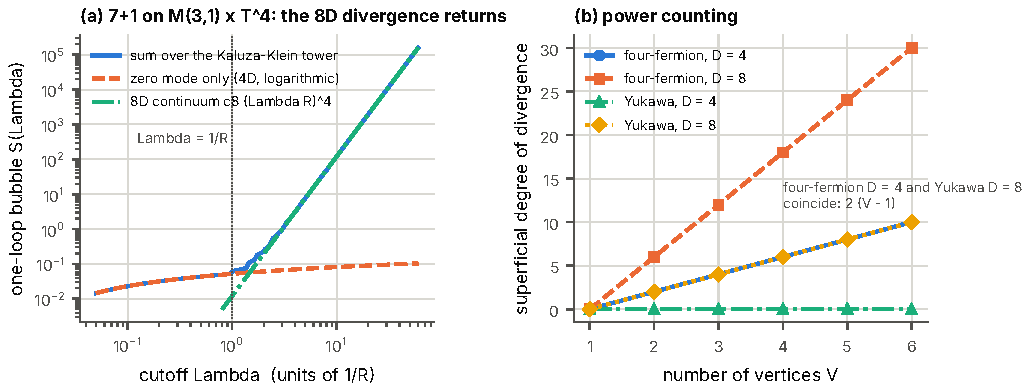
\includegraphics[width=0.92\textwidth]{../figures/fig_ng_renorm.pdf}
\caption{(a) The one-loop bubble on $7+1$ with a torus fibre of radius $R_{\rm NG}$ ($m_{\rm NG}R_{\rm NG}=0.01$),
summed over the Kaluza-Klein tower ($\mathcal B_{\rm NG}$, blue), compared with the bubble of the zero
mode alone ($f_{\rm NG}$, orange; logarithmic, four-dimensional) and with the eight-dimensional form
$\mathcal C^{(8)}_{\rm NG}(\Lambda_{\rm NG}R_{\rm NG})^4$ (green). Above $\Lambda_{\rm NG}=1/R_{\rm NG}$ the
eight-dimensional divergence returns. (b) The superficial degree of divergence $\deg_{\rm NG}$ versus the
number $\mathcal V_{\rm NG}$ of vertices. In the figure, B, f, C8, Lambda, R and nvert are
$\mathcal B_{\rm NG}$, $f_{\rm NG}$, $\mathcal C^{(8)}_{\rm NG}$, $\Lambda_{\rm NG}$, $R_{\rm NG}$ and
$\mathcal V_{\rm NG}$, and M(3,1) x T\^{}4 is the combined manifold with a torus fibre. Data:
\texttt{data/ng\_kk\_bubble.csv}, \texttt{data/ng\_superficial\_degree.csv}.}
\label{fig:renorm}
\end{figure*}

\subsection{A geometric fibre: the Kaluza-Klein tower}

If the fibre is a torus of radius $R_{\rm NG}$ on which the fields depend, each field of $7+1$ is a tower of
four-dimensional fields with the masses $(m^{\rm eff}_{\rm NG})^2=m_{1671}^2+\ell_{\rm NG}/R_{\rm NG}^2$ of
Eq.~(\ref{eq:kkmass}), where $\ell_{\rm NG}=\sum_a(n^a_{\rm NG})^2$ is the squared length of the integer
vector $(n^0_{\rm NG},n^5_{\rm NG},n^6_{\rm NG},n^7_{\rm NG})$. The number of integer vectors of squared length
$\ell_{\rm NG}$ is given by Jacobi's four-square theorem: $\mathrm r_4(\ell_{\rm NG})=8$ times the sum of the
divisors of $\ell_{\rm NG}$ that are not multiples of 4, and $\mathrm r_4(0)=1$ (check R-3 compares it with
a direct count). As a measure of the divergences we take the one-loop bubble of one four-dimensional
field of mass $m^{\rm eff}_{\rm NG}$, the integral over the Euclidean four-momentum $\varkappa_{\rm NG}$ of the
world (cut off at $\Lambda_{\rm NG}$) of the product of two propagators,
\begin{align}
&f_{\rm NG}\big((m^{\rm eff}_{\rm NG})^2\big)=\int_{\varkappa_{\rm NG}<\Lambda_{\rm NG}}\frac{d^4\varkappa_{\rm NG}}{(2\pi)^4}
\frac1{(\varkappa^2_{\rm NG}+(m^{\rm eff}_{\rm NG})^2)^2}\nonumber\\
&\ =\frac1{16\pi^2}\Big[\ln\Big(1+\frac{\Lambda_{\rm NG}^2}
{(m^{\rm eff}_{\rm NG})^2}\Big)-\frac{\Lambda_{\rm NG}^2}{\Lambda_{\rm NG}^2+(m^{\rm eff}_{\rm NG})^2}\Big],
\label{eq:bubble}
\end{align}
which grows only logarithmically, $\Lambda_{\rm NG}\,df_{\rm NG}/d\Lambda_{\rm NG}=2\Lambda_{\rm NG}^4/[16\pi^2
(\Lambda_{\rm NG}^2+(m^{\rm eff}_{\rm NG})^2)^2]\to1/(8\pi^2)$: the divergence of a dimensionless coupling in four
dimensions. Summed over the tower up to the cutoff, i.e.\ over $\ell_{\rm NG}\le(\Lambda_{\rm NG}R_{\rm NG})^2$,
\begin{equation}
\mathcal B_{\rm NG}(\Lambda_{\rm NG})=\sum_{\ell_{\rm NG}}\mathrm r_4(\ell_{\rm NG})\,
f_{\rm NG}\big(m_{1671}^2+\ell_{\rm NG}/R_{\rm NG}^2\big).
\label{eq:tower}
\end{equation}
For $\Lambda_{\rm NG}<1/R_{\rm NG}$ only the zero mode contributes, and $\mathcal B_{\rm NG}$ is the
logarithmic bubble of four dimensions (check R-4: its logarithmic slope at $\Lambda_{\rm NG}=0.3/R_{\rm NG}$
is {{GEN:kk_slope_ratio}} times $1/(8\pi^2)$). For $\Lambda_{\rm NG}\gg1/R_{\rm NG}$ the sum over integer
vectors becomes $R^4_{\rm NG}$ times an integral over the fibre momentum, whose four-dimensional volume
element is $2\pi^2$ times the cube of its length times its differential; with
$\varpi_{\rm NG}$ the ratio of that length to $\Lambda_{\rm NG}$, and for $m_{1671}\to0$,
\begin{align}
\mathcal B_{\rm NG}&\to(\Lambda_{\rm NG}R_{\rm NG})^4\,\mathcal C^{(8)}_{\rm NG},\nonumber\\
\mathcal C^{(8)}_{\rm NG}&=\frac18\int_0^1d\varpi_{\rm NG}\,\varpi_{\rm NG}^3\Big[\ln\big(1+\varpi_{\rm NG}^{-2}\big)
-\frac1{1+\varpi_{\rm NG}^2}\Big]\nonumber\\
&={{GENM:C8}},
\label{eq:c8}
\end{align}
the quartic divergence of the bubble in eight dimensions, whose integrand falls off only like the
inverse fourth power of the eight-dimensional momentum. The program finds
$\mathcal B_{\rm NG}/(\Lambda_{\rm NG}R_{\rm NG})^4=${{GEN:B_over_LR4}} at $\Lambda_{\rm NG}R_{\rm NG}=60$ (ratio
{{GEN:B_ratio}} to $\mathcal C^{(8)}_{\rm NG}$; check R-4, Fig.~\ref{fig:renorm}a). Below the
Kaluza-Klein scale $1/R_{\rm NG}$ the theory is four-dimensional; above it every mode of the tower takes
part, and the divergence of the eight-dimensional theory returns. \emph{A geometric fibre does not make
the theory renormalizable; it only postpones the eight-dimensional behaviour to the scale
$1/R_{\rm NG}$.}

On $4+4$ a geometric fibre is worse: the masses $(m^{\rm eff}_{\rm NG})^2=m_{1644}^2+[(n^0_{\rm NG})^2-
\sum_t(n^t_{\rm NG})^2]/R^2_{\rm NG}$ are negative for most modes (Fig.~\ref{fig:kk}), the number of tachyonic
modes below the cutoff grows like $(\Lambda_{\rm NG}R_{\rm NG})^4$ ({{GEN:tach10}} at
$\Lambda_{\rm NG}R_{\rm NG}=10$ and {{GEN:tach20}} at 20, ratio {{GEN:tach_ratio}}; check R-5), and the
Euclidean bubble $f_{\rm NG}$ does not exist for $(m^{\rm eff}_{\rm NG})^2<0$: the vacuum is unstable.

\subsection{The internal reading, and the verdict}

In the internal reading the fields do not depend on the fibre coordinates, and the theory is a
four-dimensional theory ($D=3$) of the four Dirac fields of Sec.~\ref{sec:superfluid}, with the
internal symmetry $\mathfrak{so}(4)$ that comes from the eight-dimensional Lorentz group. Its four-fermion
interaction is still non-renormalizable, but only mildly so, like the model of Nambu and
Jona-Lasinio, and it has a renormalizable completion: the pair amplitudes $\Delta^a_{\rm NG}$ become an
elementary complex scalar field, a vector of the fibre algebra with kinetic and quartic terms of its own
and the Yukawa coupling $\Delta^{a*}_{\rm NG}\psi^T_{\rm NG}\mathsf K^a_{\rm NG}\psi_{\rm NG}+{\rm h.c.}$; for $D=3$
the Yukawa and quartic couplings are dimensionless, and the theory is renormalizable by power counting
(checks R-1, R-2). The four-fermion model of Sec.~\ref{sec:superfluid} is the limit of this theory in which
the scalar field has no kinetic term at the scale $\Lambda_{\rm NG}$.

The answer to the question of the task is therefore: \emph{the combined manifolds do not cure the
non-renormalizability of the eight-dimensional theory.} With a geometric fibre the theory is
eight-dimensional above $1/R_{\rm NG}$ and as non-renormalizable as before ($7+1$) or inconsistent
($4+4$). With an internal fibre the problem disappears only because the theory is no longer
eight-dimensional: it is a four-dimensional theory with an internal symmetry inherited from the
eight-dimensional Lorentz group, and it is renormalizable in its Yukawa form, as any four-dimensional
theory of fermions and scalars with these couplings is.
